\documentclass[11pt,a4paper]{article}

\usepackage{fullpage}
\usepackage{hyperref}
\usepackage{graphicx}
\usepackage{float}

\usepackage{fancyhdr}
\pagestyle{fancy}
\fancyhf{}
\usepackage{todonotes}                %% notes from the authors

\renewcommand{\headrulewidth}{0pt}
\renewcommand{\footrulewidth}{0pt}

\newcommand*{\escape}[1]{\texttt{\textbackslash#1}}

\fancypagestyle{firstpagefooter} {
	\lfoot{\tiny{Version: 25.09.2018}}
	\cfoot{}
	\rfoot{\thepage}
	
}

\lfoot{Name: Mohammed Ajil Legi: 11-948-734}
\rfoot{\thepage}

\begin{document}

\title{Advanced Systems Lab Report\\ \normalsize{Autumn Semester 2018}}
\author{Name: Mohammed Ajil\\Legi: 11-948-734}
\date{
	\vspace{4cm}
	\textbf{Grading} \\
	\vspace{0.5cm}
	\begin{tabular}{|c|c|}
		\hline  \textbf{Section} & \textbf{Points} \\
		\hline  1                &                 \\ 
		\hline  2                &                 \\ 
		\hline  3                &                 \\ 
		\hline  4                &                 \\ 
		\hline  5                &                 \\ 
		\hline  6                &                 \\ 
		\hline  7                &                 \\ 
		\hline \hline Total      &                 \\
		\hline 
	\end{tabular} 
}
\maketitle
\thispagestyle{firstpagefooter}

\newpage

\section{System Overview (75 pts)}
%
\subsection{Class Overview}
%
\begin{figure}[H]
    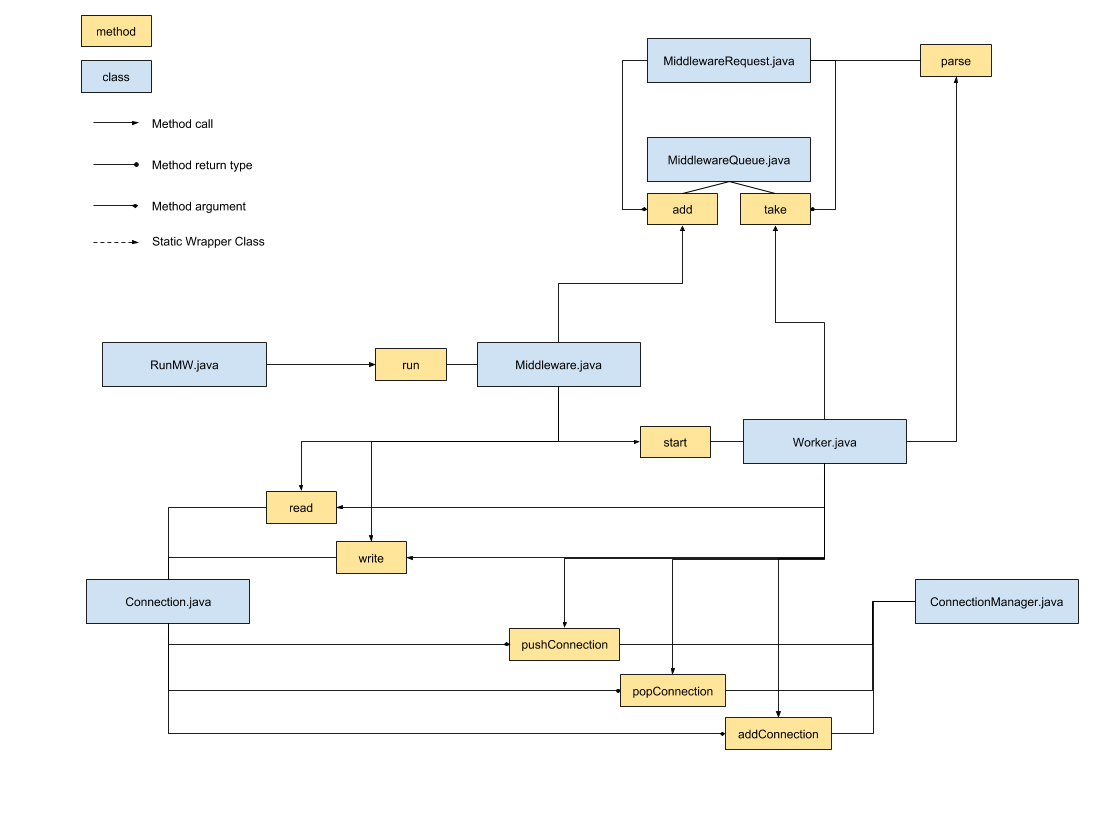
\includegraphics[width=\linewidth]{../illustrations/class_diagram.png}
    \caption{Class Diagram}
    \label{fig:class_diagram}
\end{figure}
%
We will start by looking at a class diagram of the middleware.
%
In \ref{fig:class_diagram} we can see all the classes that compose the middleware.
%
The system is represented in its running state, i.e. all methods that are only used when starting up are omitted.
%
In the following paragraphs we will look at each of the components in detail.
%
\paragraph{\texttt{RunMW.java}}
%
This class has a single responsibility. It parses the command line arguments and runs the middleware thread using these.
%
\paragraph{\texttt{MiddlewareRequest.java}}
%
This class represents a request coming from a client.
%
The object holds all the relevant data of the request, i.e. all time measurements, whether or not the request was successful and the \texttt{Connection} object of the client that sent the request.
%
In this class we implement the parsing method, that scans the command string and populates fields in the object.
%
If the middleware is running in sharded mode, Multi-Get requests will be sharded into a list of commands.
%
\paragraph{\texttt{Middleware.java}}
%
This class represents the net thread of the system. Its responsibilities are first to accept client connections and register them so that we can start accepting requests. 
%
Second the thread also reads requests from already acccepted client connections and enqueues them in the \texttt{MiddlewareQueue}.
%
To avoid busy waiting and accessing client sockets that do not have data to read we use a \texttt{Selector}. 
%
Basically this is a mechanism that allows us to register connections and the selector will deliver only the connections that have data ready to read.
%
We also register the server socket with the selector and receive connections that are ready to be accepted.
%
Using this we can maximize the utilization of the CPU time used by the net thread.
%
We will look at the process of accepting connections and requests in detail in section~\ref{subsec:handlingRequests}
%
\paragraph{\texttt{MiddlewareQueue.java}}
%
In this middleware the \texttt{MiddlewareQueue} is a first class citizen, as are the workers and the net thread.
%
This decision is made based on the fact that the queue should not be owned by either the net or the worker threads.
%
The queue is not much more than a static wrapper around a \texttt{BlockingQueue}.
%
The access to take a request out of the queue is synchronized, so that we avoid processing the same request twice.
%
\paragraph{\texttt{Worker.java}}
%
In this class the actual processing of the request is done.
%
Depending on the type of the request that worker threads handle them differently. 
%
This will be adressed in detail in section~\ref{subsec:handlingRequests}.
%
In general a worker thread takes a request out of the \texttt{MiddlewareQueue}, after that the worker calls the parse method offered by \texttt{MiddlewareRequest}.
%
After that several new fields in the request object are populated, such as \texttt{RequestType} for example.
%
The parsed request will then be scheduled on the memcached servers depending on the server mode and request type.
%
The worker then waits for the responses from the memcached servers, parses the responses and then sends the appropriate response to the client.
%
After finishing processing the request the worker will then log the relevant fields for the analysis in a CSV format.
%
\paragraph{\texttt{Connection.java}}
%
The connection class is a convenience wrapper around a \texttt{SocketChannel}.
%
It represents both the client and server connections.
%
It allows us to specify if a connection should be blocking or not.
%
The goal of this class is that when using a connection we do not need to care about the configuration and how to read from the socket, instead we can just call the \texttt{read()} method and the different modes are handled internally.
%
\paragraph{\texttt{ServerManager.java}}
%
This class is used by the worker threads.
%
The \texttt{ServerManager} holds the \texttt{Connection} objects for the memcached servers.
%
This class offers the method \texttt{getConnection(int i)}, which will return the appropriate server connection based on the integer that is passed, such that the load is scheduled in a round robin fashion.
%
We will see in \ref{subsec:handlingRequests} how exactly that is handled based on the Id of the request.
%
Even if the request will go to all memcached servers it still makes sense to choose the first server to send the request to based on round robin.
%
This distributes the load even if we only have Set requests.
%
\subsection{Message Parsing}
%
As mentioned before the first thing the workers do with the request is parse it.
%
Parsing means mainly two things here, first we will determine the type of request we are looking, this tells us how to further handle the request.
%
Second, if applicable, we set the Multi-Get Size.
%
In the specific case of running the server in sharded mode and receiving a Multi-Get Request we will split the keys in the request and depending on the Multi-Get Size and number of servers populate a list of commands, this is known as "sharding" a command.
%
The number of shards is exactly \texttt{min(multiGetSize, numServers)}
%
\subsection{Response Parsing}
%
In two cases, specifically when handling sharded Multi-Get or Set requests we need to do some work before sending the request to the client.
%
\\
%
In the case of Set requests we need to make sure that the key was set on all the three servers.
%
That can be achieved by simply checking if all the responses equal \texttt{STORED\escape{r}\escape{n}}.
%
If that is the case we send the same response back to the client.
%
If not, it does not matter if we receive an error or if the key was simply not stored on some or all servers, we respond to the client with \texttt{NOT STORED\escape{r}\escape{n}} to let the client know that it should retry setting the key.
%
\\
%
In the case of sharded Multi-Get requests we need to combine the responses from all servers back to a single response and send it back to the client.
%
This is done by simply removing the end marker from all responses, concatenating them and then adding the end marker back at the end.
%
Finally we count the keys and record how many keys we have received to be able to calculate the miss rate and then we send the response on its way to the client.
%
\subsection{Logs}
%
To handle the logs in this multithreaded setting we use \texttt{log4j}.
%
The logs from all the workers are consolidated into a single CSV file per middleware, this is handled by \texttt{log4j}.
%
After finishing processing a request the workers will call the \texttt{toString()} method implemented by the \texttt{MiddlewareRequest} to produce a CSV log line.
%
This log line is passed to \texttt{log4j}.
%
\subsection{Queues}
%
\begin{figure}[H]
    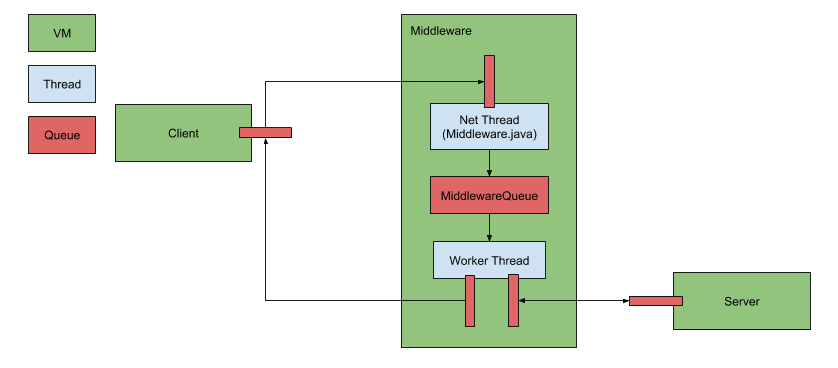
\includegraphics[width=\linewidth]{../illustrations/threads_and_queues.png}
    \caption{Threads and Queues}
    \label{fig:threads_and_queues}
\end{figure}
%
In figure~\ref{fig:threads_and_queues} we can see an illustration of threads and queues in the system.
%
The arrow directions indicate the flow of requests.
%
Arrows connecting different VMs represent sockets, thus the all queues except the MiddlewareQueue refer to socket queues.
%
The illustration only shows one instance of a client, a server, and a worker thread.
%
In the full system there are three instances of clients and servers.
%
Depending on the configuration there are also many worker threads.
%
The queues and connections for these variable components are also replicated for the number of instances.
%
\subsection{Handling Requests}\label{subsec:handlingRequests}
%
In this section we go into detail on how the middleware handles incoming connections and how the different types of requests are handled by the middleware.
%
What follows are sequence diagrams that model the behaviour of the system for different request types.
%
Important to note here, that again the system is assumed to be in a running state, all the setup methods are executed.
%
Further there are some simplifications and abstractions in the diagrams to reduce clutter, for example not listing all arguments to a method call.
%
Also not all method calls are illustrated, only the ones that are relevant on how we handle different requests.
%
These abstractions should not impact the understanding of the middleware, I tried to design them as self explanatory as possible.
%
Finally the sequence diagrams model the handling of one request, therefore we model only one client and one worker.
%
\begin{figure}[H]
    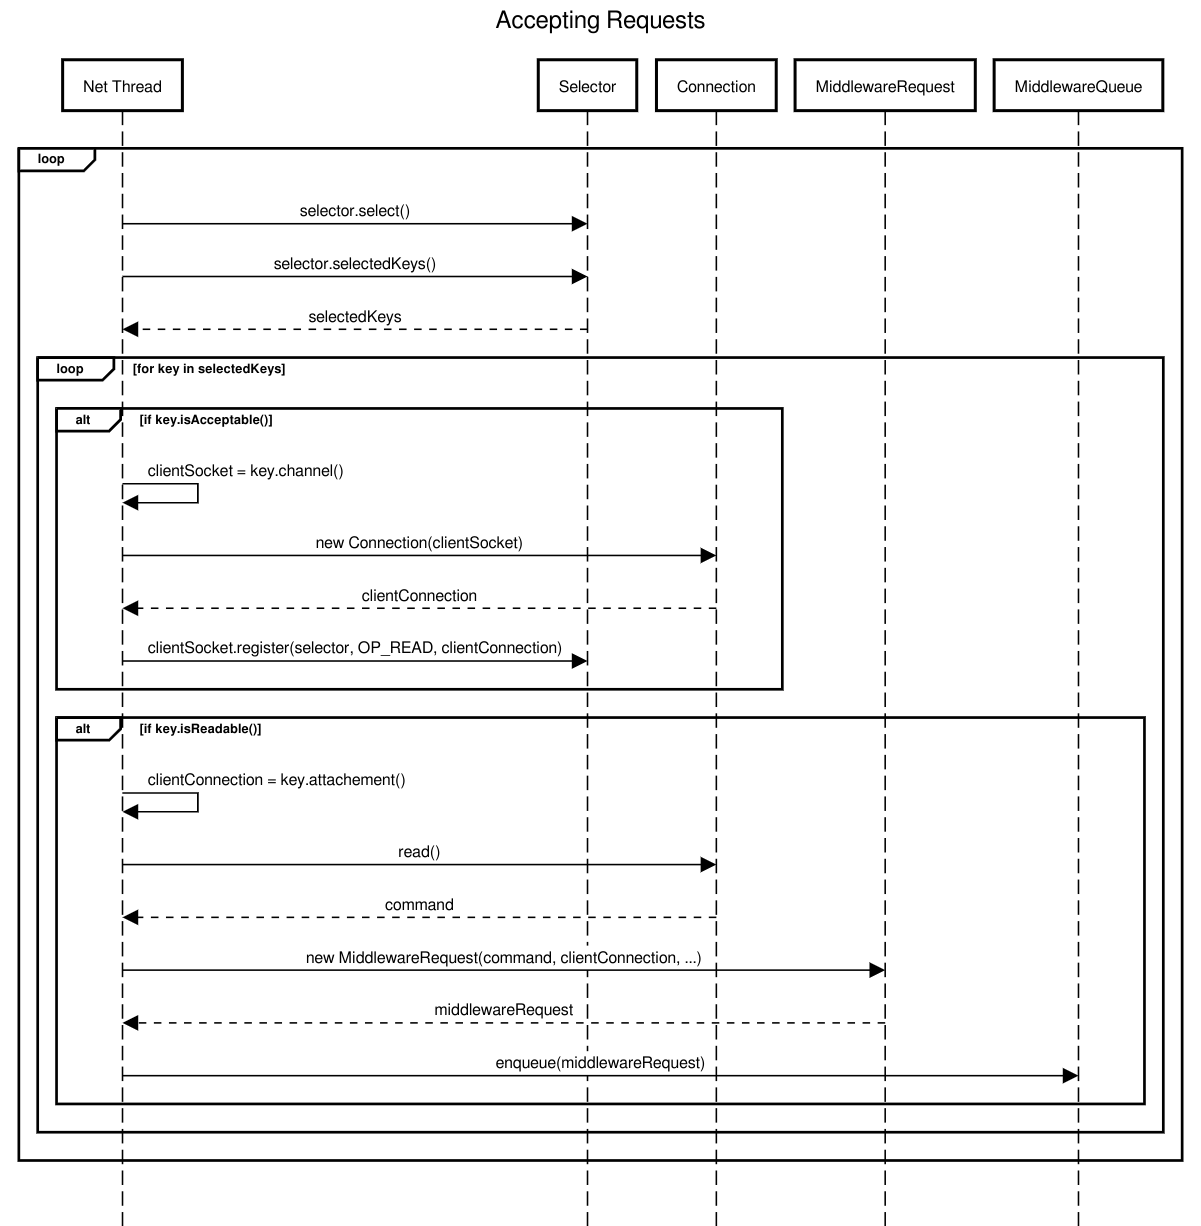
\includegraphics[width=\linewidth]{../illustrations/accepting_requests.png}
    \caption{Accepting new connections and requests}
    \label{fig:accepting_requests}
\end{figure}
%
\begin{figure}[H]
    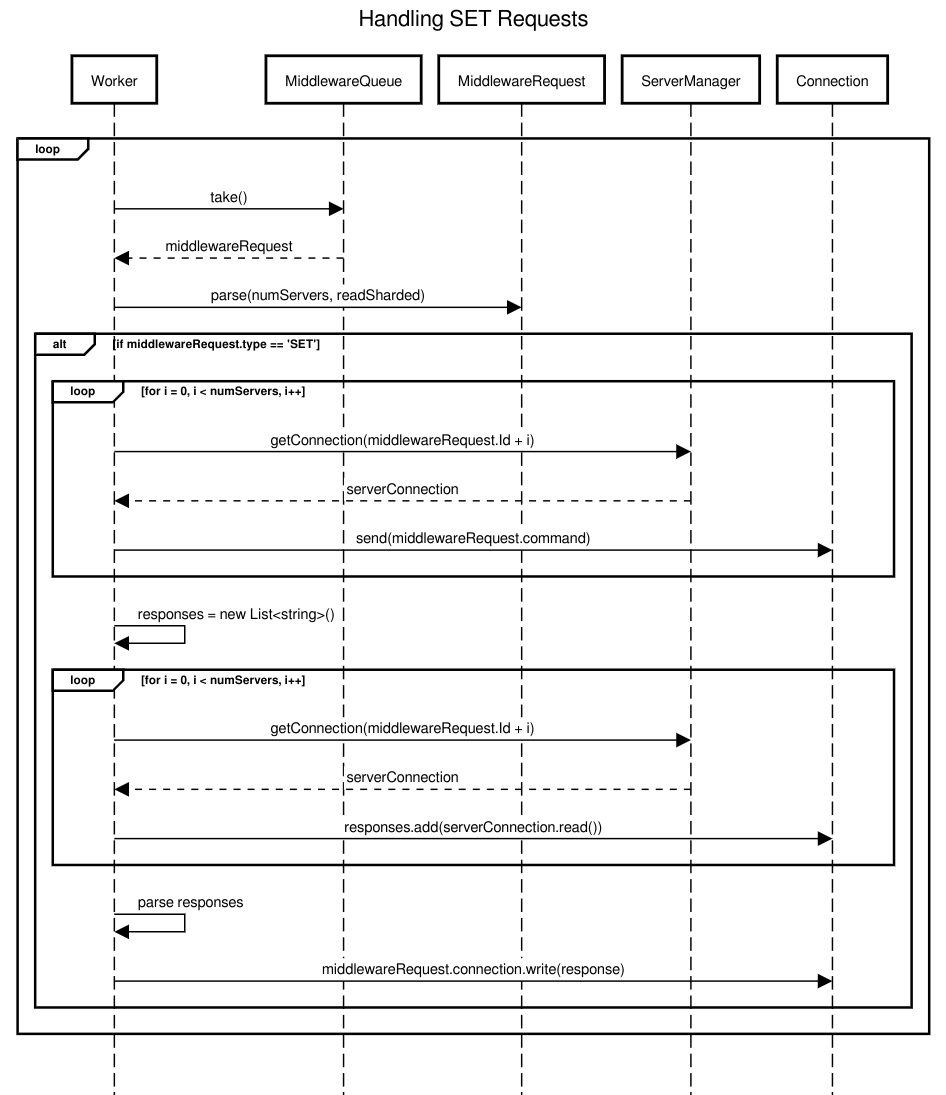
\includegraphics[width=\linewidth]{../illustrations/handling_set.png}
    \caption{Handling Set requests}
    \label{fig:handling_set}
\end{figure}
%
\begin{figure}[H]
    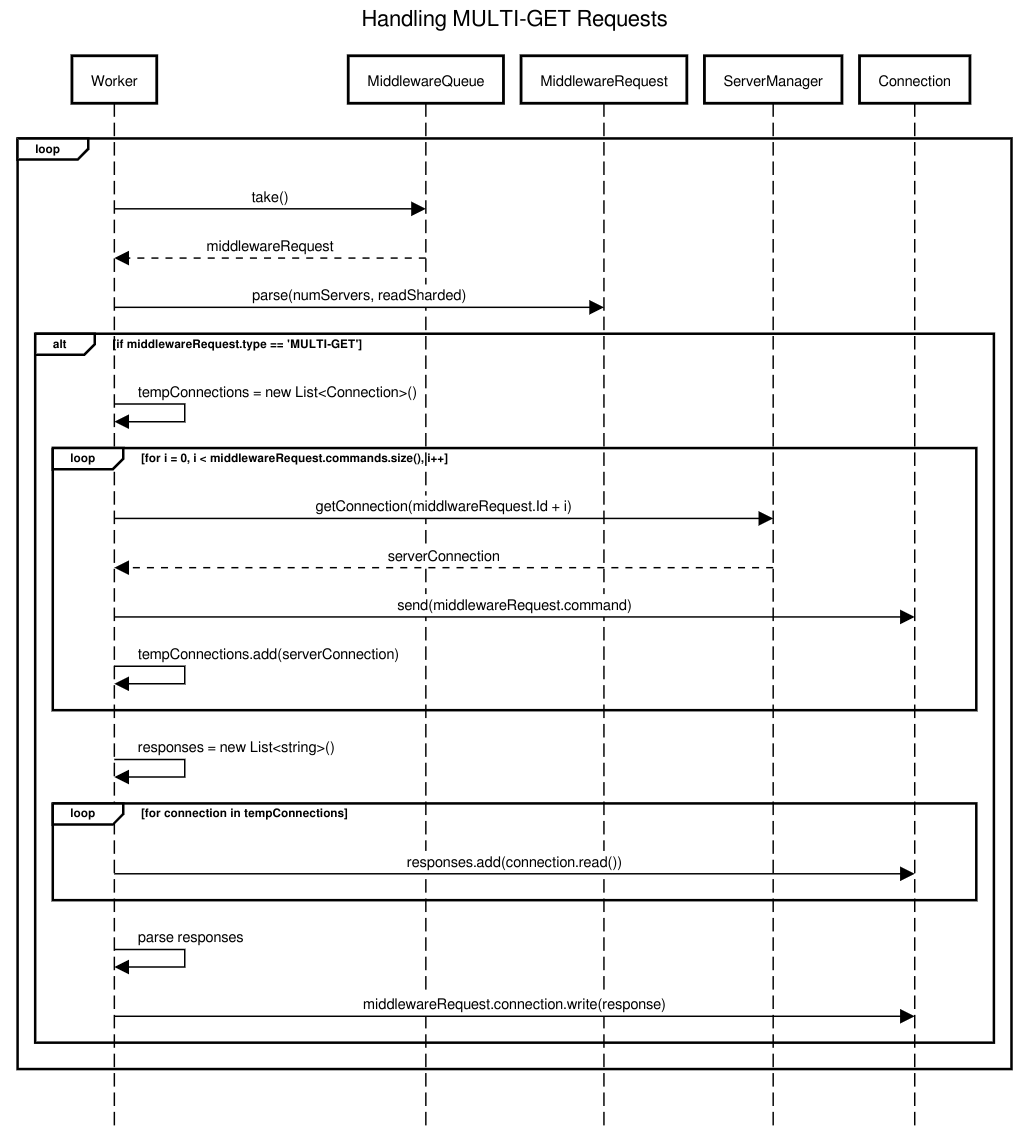
\includegraphics[width=\linewidth]{../illustrations/handling_mget.png}
    \caption{Handling Multi-Get requests}
    \label{fig:handling_mget}
\end{figure}
%
\begin{figure}[H]
    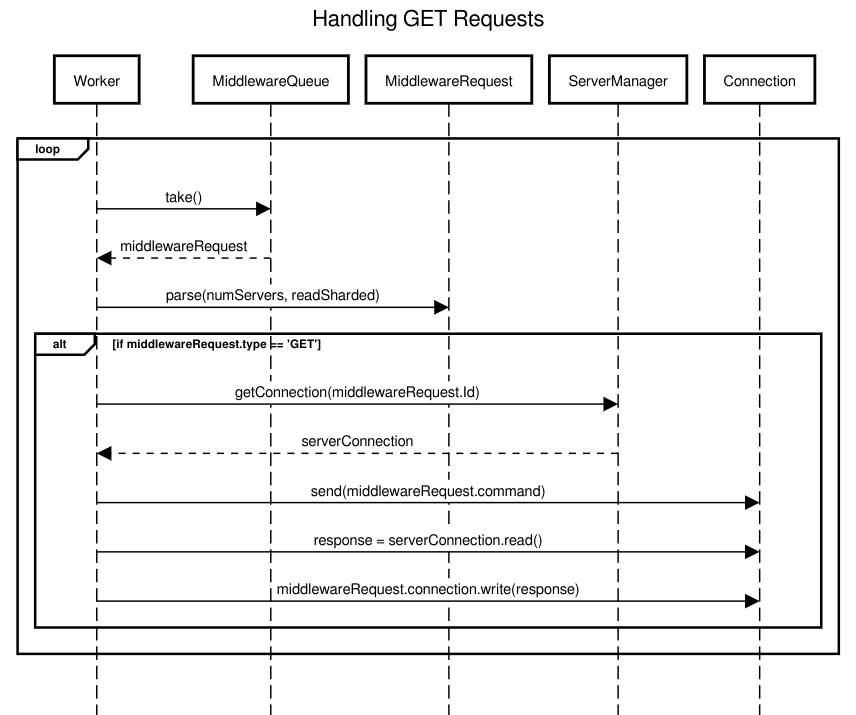
\includegraphics[width=\linewidth]{../illustrations/handling_get.png}
    \caption{Handling Get requests}
    \label{fig:handling_get}
\end{figure}
%
\subsection{Measurements}
%
Before getting into the analysis I want to lose a few words on the measurements and how they are handled.
%
\paragraph{No Middleware}
%
In this case we rely entirely on the output of \texttt{memtier\_benchmark}.
%
There we receive detailed numbers on number of requests and latency, however aggregated per one second intervals.
%
\paragraph{Middleware}
%
In this case we can use the detailed measurements from the middleware logs to produce the plots.
%
The measurements use \texttt{System.nanoTime()} in combination with \\ \texttt{System.currentTimeMillis()} to produce nanosecond Unix Timestamps.
%
We can compute the response time for each request and aggregate the average over all the requests.
%
When computing the average throughput we create a histogram based on the time a request was completed with the same number of bins as the duration of the experiment in seconds.
%
After that we sum these values over all middlewares and compute the average over the seconds the experiments was running.
%
All the plots use the 95\% percent confidence interval as an error measure.

\section{Baseline without Middleware (75 pts)}

In this experiments you study the performance characteristics of the memtier clients and memcached servers.

\subsection{One Server}

Both, for a read-only and write-only workload plot the throughput and the response time as a function of NumClients. All clients are connected to a single memcached instance.

Use 3 load generating VMs, with one memtier (CT=2) each, and vary the number of virtual clients (VC) per memtier thread between 1 and 32. Show how the behavior of the server changes as we add more clients.

\begin{center}
	\scriptsize{
		\begin{tabular}{|l|c|}
			\hline Number of servers                & 1                        \\ 
			\hline Number of client machines        & 3                        \\ 
			\hline Instances of memtier per machine & 1                        \\ 
			\hline Threads per memtier instance     & 2                        \\
			\hline Virtual clients per thread       & [1..32]                  \\ 
			\hline Workload                         & Write-only and Read-only \\
			\hline Multi-Get behavior               & N/A                      \\
			\hline Multi-Get size                   & N/A                      \\
			\hline Number of middlewares            & N/A                      \\
			\hline Worker threads per middleware    & N/A                      \\
			\hline Repetitions                      & 3 or more                \\ 
			\hline 
		\end{tabular}
	} 
\end{center}

\subsubsection{Explanation}

Describe in which phase the memcached servers are under-saturated, saturated, or over-saturated. Describe how throughput and response time correlate. Explain what further conclusions can be drawn from the experiment.


\subsection{Two Servers}

For a read-only and write-only workload plot throughput and response time as a function of NumClients. The clients are connected to two memcached instances. 

Use 1 load generating VM, with one memtier (CT=1) connected to each memcached instance (two memcache instances in total), and vary the number of virtual clients (VC) per memtier thread between 1 and 32. Show how the behavior of the server changes and explain what conclusions we can draw from this experiment.

\begin{center}
	\scriptsize{
		\begin{tabular}{|l|c|}
			\hline Number of servers                & 2                        \\ 
			\hline Number of client machines        & 1                        \\ 
			\hline Instances of memtier per machine & 2                        \\ 
			\hline Threads per memtier instance     & 1                        \\
			\hline Virtual clients per thread       & [1..32]                  \\ 
			\hline Workload                         & Write-only and Read-only \\
			\hline Multi-Get behavior               & N/A                      \\
			\hline Multi-Get size                   & N/A                      \\
			\hline Number of middlewares            & N/A                      \\
			\hline Worker threads per middleware    & N/A                      \\
			\hline Repetitions                      & 3 or more (at least 1 minute each)                \\ 
			\hline 
		\end{tabular}
	} 
\end{center}

\subsubsection{Explanation}

Describe how this experiment compares to the previous section. Which results are the same and which ones differ? Explain what further conclusions can be drawn from the experiment.


\subsection{Summary}

Based on the experiments above, fill out the following table:

\begin{center}
	{Maximum throughput of different VMs.}
	\begin{tabular}{|l|p{2cm}|p{2cm}|p{4cm}|}
		\hline                        & Read-only workload & Write-only workload & Configuration gives max. throughput \\ 
		\hline One memcached server   &                    &                     &                                     \\ 
		\hline One load generating VM &                    &                     &                                     \\ 
		\hline 
	\end{tabular}
\end{center}


Write at least two paragraphs about how both results relate. Describe what is the bottleneck of this setup is. If the maximum throughput for both experiments is the same, explain why. If it is not the case, explain why not. Write down key take-away messages about the behaviour of the memtier clients and the memcached servers.

\section{Baseline with Middleware (90 pts)}

In this set of experiments, you will have to use three load generator VMs and 1 memcached server, measuring how the throughput of the system changes when increasing the number of clients. Scaling virtual clients inside memtier has to be done as explained in the previous sections. Plot both throughput and response time as measured on the middleware.

\subsection{One Middleware}

Connect three load generator machines (one instance of memtier with CT=2) to a single middleware and use 1 memcached server. Run a read-only and a write-only workload with increasing number of clients (between 2 and 64) and measure response time \emph{both at the client and at the middleware}, and plot the throughput and response time measured in the middleware.

Repeat this experiment for different number of worker threads inside the middleware: 8, 16, 32, 64.

\begin{center}
	\scriptsize{
		\begin{tabular}{|l|c|}
			\hline Number of servers                & 1                        \\ 
			\hline Number of client machines        & 3                        \\ 
			\hline Instances of memtier per machine & 1                        \\ 
			\hline Threads per memtier instance     & 2                        \\
			\hline Virtual clients per thread       & [1..32]                  \\ 
			\hline Workload                         & Write-only and Read-only \\
			\hline Multi-Get behavior               & N/A                      \\
			\hline Multi-Get size                   & N/A                      \\
			\hline Number of middlewares            & 1                        \\
			\hline Worker threads per middleware    & [8..64]                  \\
			\hline Repetitions                      & 3 or more (at least 1 minute each)                \\ 
			\hline 
		\end{tabular}
	} 
\end{center}

\subsubsection{Explanation}

Provide a detailed analysis of the results (e.g., bottleneck analysis, component utilizations, average queue lengths, system saturation). Add any additional figures and experiments that help you illustrate your point and support your claims.

\subsection{Two Middlewares}

Connect three load generator machines (two instances of memtier with CT=1) to two middlewares and use 1 memcached server. Run a read-only and a write-only workload with increasing number of clients (between 2 and 64) and measure response time \emph{both at the client and at the middleware}, and plot the throughput and response time as measured in the middleware.

Repeat this experiment for different number of worker threads inside the middleware: 8, 16, 32, 64.

\begin{center}
	\scriptsize{
		\begin{tabular}{|l|c|}
			\hline Number of servers                & 1                        \\ 
			\hline Number of client machines        & 3                        \\ 
			\hline Instances of memtier per machine & 2                        \\ 
			\hline Threads per memtier instance     & 1                        \\
			\hline Virtual clients per thread       & [1..32]                  \\ 
			\hline Workload                         & Write-only and Read-only \\
			\hline Multi-Get behavior               & N/A                      \\
			\hline Multi-Get size                   & N/A                      \\
			\hline Number of middlewares            & 2                        \\
			\hline Worker threads per middleware    & [8..64]                  \\
			\hline Repetitions                      & 3 or more (at least 1 minute each)                \\ 
			\hline 
		\end{tabular}
	} 
\end{center}

\subsubsection{Explanation}

Provide a detailed analysis of the results (e.g., bottleneck analysis, component utilizations, average queue lengths, system saturation). Add any additional figures and experiments that help you illustrate your point and support your claims.

\subsection{Summary}

Based on the experiments above, fill out the following table. For both of them use the numbers from a single experiment to fill out all lines. Miss rate represents the percentage of GET requests that return no data. Time in the queue refers to the time spent in the queue between the net-thread and the worker threads.


\begin{center}
	{Maximum throughput for one middleware.}
	\begin{tabular}{|l|p{2cm}|p{2cm}|p{2cm}|p{2cm}|}
		\hline                                & Throughput & Response time & Average time in queue & Miss rate \\ 
		\hline Reads: Measured on middleware  &            &               &                       &           \\ 
		\hline Reads: Measured on clients     &            &               & n/a                   &           \\ 
		\hline Writes: Measured on middleware &            &               &                       & n/a       \\ 
		\hline Writes: Measured on clients    &            &               & n/a                   & n/a       \\ 
		\hline 
	\end{tabular}
\end{center}

\begin{center}
	{Maximum throughput for two middlewares.}
	\begin{tabular}{|l|p{2cm}|p{2cm}|p{2cm}|p{2cm}|}
		\hline                                & Throughput & Response time & Average time in queue & Miss rate \\ 
		\hline Reads: Measured on middleware  &            &               &                       &           \\ 
		\hline Reads: Measured on clients     &            &               & n/a                   &           \\ 
		\hline Writes: Measured on middleware &            &               &                       & n/a       \\ 
		\hline Writes: Measured on clients    &            &               & n/a                   & n/a       \\ 
		\hline 
	\end{tabular}
\end{center}

Based on the data provided in these tables, write at least two paragraphs summarizing your findings about the performance of the middleware in the baseline experiments.

\section{Throughput for Writes (90 pts)}

\subsection{Full System}

Connect three load generating VMs to two middlewares and three memchached servers. Run a write-only experiment. 
You need to plot throughput and response time measured on the middleware as a function of number of clients. The measurements have to be performed for 8, 16, 32 and 64 worker threads inside each middleware.

\begin{center}
	\scriptsize{
		\begin{tabular}{|l|c|}
			\hline Number of servers                & 3          \\ 
			\hline Number of client machines        & 3          \\ 
			\hline Instances of memtier per machine & 2          \\ 
			\hline Threads per memtier instance     & 1          \\
			\hline Virtual clients per thread       & [1..32]    \\ 
			\hline Workload                         & Write-only \\
			\hline Multi-Get behavior               & N/A        \\
			\hline Multi-Get size                   & N/A        \\
			\hline Number of middlewares            & 2          \\
			\hline Worker threads per middleware    & [8..64]    \\
			\hline Repetitions                      & 3 or more (at least 1 minute each)  \\ 
			\hline 
		\end{tabular}
	} 
\end{center}

\subsubsection{Explanation}

Provide a detailed analysis of the results (e.g., bottleneck analysis, component utilizations, average queue lengths, system saturation). Add any additional figures and experiments that help you illustrate your point and support your claims.

\subsection{Summary}

Based on the experiments above, fill out the following table with the data corresponding to the maximum throughput point for all four worker-thread scenarios.

\begin{center}
	{Maximum throughput for the full system}
	\begin{tabular}{|l|p{1.5cm}|p{1.5cm}|p{1.5cm}|p{1.5cm}|}
		\hline                                            & WT=8 & WT=16 & WT=32 & WT=64 \\ 
		\hline Throughput (Middleware)                    &      &       &       &       \\ 
		\hline Throughput (Derived from MW response time) &      &       &       &       \\ 
		\hline Throughput (Client)                        &      &       &       &       \\ 
		\hline Average time in queue                      &      &       &       &       \\ 
		\hline Average length of queue                    &      &       &       &       \\ 
		\hline Average time waiting for memcached         &      &       &       &       \\ 
		\hline 
	\end{tabular}
\end{center}

Based on the data provided in these tables, draw conclusions on the state of your system for a variable number of worker threads.

\section{Gets and Multi-gets (90 pts)}

For this set of experiments you will use three load generating machines, two middlewares and three memcached servers. Each memtier instance should have 2 virtual clients in total and the number of middleware worker threads is 64, or the one that provides the highest throughput in your system (whichever number of threads is smaller).

For multi-GET workloads, use the \texttt{--ratio} parameter to specify the exact ratio between SETs and GETs. You will have to measure response time on the client as a function of multi-get size, with and without sharding on the middlewares.

\subsection{Sharded Case}

Run multi-gets with 1, 3, 6 and 9 keys (memtier configuration) with sharding enabled (multi-gets are broken up into smaller multi-gets and spread across servers). Plot average response time as measured on the client, as well as the 25th, 50th, 75th, 90th and 99th percentiles.

\begin{center}
	\scriptsize{
		\begin{tabular}{|l|c|}
			\hline Number of servers                & 3                       \\ 
			\hline Number of client machines        & 3                       \\ 
			\hline Instances of memtier per machine & 2                       \\ 
			\hline Threads per memtier instance     & 1                       \\
			\hline Virtual clients per thread       & 2     		            \\ 
			\hline Workload                         & ratio=1:$<$Multi-Get size$>$             \\
			\hline Multi-Get behavior               & Sharded                 \\
			\hline Multi-Get size                   & [1..9]                  \\
			\hline Number of middlewares            & 2                       \\
			\hline Worker threads per middleware    & max. throughput config. \\
			\hline Repetitions                      & 3 or more (at least 1 minute each)               \\ 
			\hline 
		\end{tabular}
	} 
\end{center}

\subsubsection{Explanation}

Provide a detailed analysis of the results (e.g., bottleneck analysis, component utilizations, average queue lengths, system saturation). Add any additional figures and experiments that help you illustrate your point and support your claims.

\subsection{Non-sharded Case}

Run multi-gets with 1, 3, 6 and 9 keys (memtier configuration) with sharding disabled. Plot average response time as measured on the client, as well as the 25th, 50th, 75th, 90th and 99th percentiles.

\begin{center}
	\scriptsize{
		\begin{tabular}{|l|c|}
			\hline Number of servers                & 3                       \\ 
			\hline Number of client machines        & 3                       \\ 
			\hline Instances of memtier per machine & 2                       \\ 
			\hline Threads per memtier instance     & 1                       \\
			\hline Virtual clients per thread       & 2                		 \\ 
			\hline Workload                         & ratio=1:$<$Multi-Get size$>$              \\
			\hline Multi-Get behavior               & Non-Sharded             \\
			\hline Multi-Get size                   & [1..9]                  \\
			\hline Number of middlewares            & 2                       \\
			\hline Worker threads per middleware    & max. throughput config. \\
			\hline Repetitions                      & 3 or more (at least 1 minute each)               \\ 
			\hline 
		\end{tabular}
	} 
\end{center}

\subsubsection{Explanation}

Provide a detailed analysis of the results (e.g., bottleneck analysis, component utilizations, average queue lengths, system saturation). Add any additional figures and experiments that help you illustrate your point and support your claims.

\subsection{Histogram}

For the case with 6 keys inside the multi-get, display four histograms representing the sharded and non-sharded response time distribution, both as measured on the client, and inside the middleware. Choose the bucket size in the same way for all four, and such that there are at least 10 buckets on each of the graphs.

\subsection{Summary}

Provide a detailed comparison of the sharded and non-shareded modes. For which multi-GET size is sharding the preferred option? Provide a detailed analysis of your system. Add any additional figures and experiments that help you illustrate your point and support your claims.

\section{2K Analysis (90 pts)}

For 3 client machines (with 64 total virtual clients per client VM) measure the throughput and response time of your system in a 2k experiment with repetitions. All GET operations have a single key. Investigate the following parameters:

\begin{itemize}
		
	\item Memcached servers: 1 and 3
	\item Middlewares: 1 and 2
	\item Worker threads per MW: 8 and 32
	      	      
\end{itemize}

Repeat the experiment for (a)~a write-only and (b)~a read-only workload.
For each of the two workloads, what is the impact of these parameters on throughput, respectively response time?

\begin{center}
	\scriptsize{
		\begin{tabular}{|l|c|}
			\hline Number of servers                & 1 and 3                                     \\ 
			\hline Number of client machines        & 3                                           \\ 
			\hline Instances of memtier per machine & 1 (1 middleware) or 2 (2 middlewares) \\ 
			\hline Threads per memtier instance     & 2 (1 middleware) or 1 (2 middlewares)   \\
			\hline Virtual clients per thread       &  32                                     \\ 
			\hline Workload                         & Write-only and Read-only\\
			\hline Multi-Get behavior               & N/A                                         \\
			\hline Multi-Get size                   & N/A                                         \\
			\hline Number of middlewares            & 1 and 2                                     \\
			\hline Worker threads per middleware    & 8 and 32                                    \\
			\hline Repetitions                      & 3 or more (at least 1 minute each)                                   \\ 
			\hline 
		\end{tabular}
	} 
\end{center}

\section{Queuing Model (90 pts)}

Note that for queuing models it is enough to use the experimental results from the previous sections. It is, however, possible that the numbers you need are not only the ones in the figures we asked for, but also the internal measurements that you have obtained through instrumentation of your middleware.

\subsection{M/M/1}

Build queuing model based on Section 4 (write-only throughput) for each worker-thread configuration of the middleware. Use one M/M/1 queue to model your entire system. Motivate your choice of input parameters to the model. Explain for which experiments the predictions of the model match and for which they do not.

\subsection{M/M/m}

Build an M/M/m model based on Section 4, where each middleware worker thread is represented as one service.  Motivate your choice of input parameters to the model. Explain for which experiments the predictions of the model match and for which they do not.

\subsection{Network of Queues}

Based on Section 3, build a network of queues which simulates your system. Motivate the design of your network of queues and relate it wherever possible to a component of your system. Motivate your choice of input parameters for the different queues inside the network. Perform a detailed analysis of the utilization of each component and clearly state what the bottleneck of your system is. Explain for which experiments the predictions of the model match and for which they do not.

\end{document}

